\documentclass[a4paper,12pt]{scrartcl}
\usepackage{verbatim}
\usepackage[utf8]{inputenc}
\usepackage[brazil]{babel}
\usepackage[margin=25mm,bottom=30mm]{geometry}
\usepackage{hyperref}
\usepackage{amsmath,amssymb}
\usepackage{algorithm}
\usepackage{algpseudocode}
\usepackage{minted}
\usepackage{tabto}
\usepackage{siunitx}
\usepackage{graphicx,url}
\usepackage{listings}
\lstset{
  language=Python,
  basicstyle=\ttfamily\small, 
  keywordstyle=\color{blue}, 
  stringstyle=\color{magenta}, 
  commentstyle=\color{red}, 
  extendedchars=true, 
  showspaces=false, 
  showstringspaces=false, 
  numbers=left,
  numberstyle=\tiny,
  breaklines=true, 
  backgroundcolor=\color{pink!10},
  breakautoindent=true, 
  captionpos=b,
  xleftmargin=0pt,
}

\newcommand{\algorithmautorefname}{Algoritmo}
\title{Trabalho de Ordenação e Estatísticas de Ordem}
\subtitle{Técnicas de Programação Avançada — Ifes -  Campus Serra - Prof.Dr. Jefferson O. Andrade}
\author{Ewerson Vieira Nascimento\\ Paulo Ricardo Viana \\ William Vaneli  }
\date{21 de Outubro de 2019}
\begin{document}
\maketitle
\tableofcontents
\section{Introdução}

Este  documento refere-se aos testes de desempenho dos algoritmos requeridos para o Trabalho de Ordenação e Estatísticas de Ordem da disciplina de Técnicas de Programação Avançada.

\begin{comment}
\section{Enunciado}

Este trabalho consiste de duas etapas:

\begin{enumerate}
\item Implementação de um conjunto de algoritmos de ordenação.
\item Análise do desempenho dos algoritmos implementados.
\end{enumerate}

A descrição destas duas etapas será vista com mais detalhes abaixo.
\end{comment}


\section{Dados para Testes}

Foram fornecidos pelo professor alguns arquivos de dados para que os algoritmos fossem testados e realizássemos as coletas dos tempos de execução para cada algoritmo. Esses arquivos de dados possuem número crescente de registros, indo de 10 até 7.500.000 registros.


\subsection{Arquivos de Dados}

Os arquivos de dados estão no formato CSV e são compostos pelos seguintes
campos:

\begin{enumerate}
\item Email (\texttt{email}); tipo: texto.
\item Sexo (\texttt{gender}); tipo: caractere; valores válidos: \texttt{M},
  \texttt{F}, \texttt{O}.
\item Identificador de Usuário (\texttt{uid}); tipo: alfa-numérico; único.
\item Data de nascimento (\texttt{birthdate}); tipo: data; formato: ISO-8601.
\item Altura, em centímetros (\texttt{height}); tipo: inteiro.
\item Peso, em quilogramas (\texttt{weight}); tipo: numérico.
\end{enumerate}

Por conta disso, criamos uma classe em Python com os mesmos atributos:
\begin{lstlisting}
class Person:
    def __init__(self, email, gender, uid, birthdate, height, weight):
        self.email = email
        self.gender = gender
        self.uid = uid
        self.birthdate = birthdate
        self.height = height
        self.weight = weight
\end{lstlisting}


\section{Implementação do Trabalho}

O trabalho foi implementado na linguagem Python, utilizando o Visual Studio Code no Ubuntu 18.04 como ambiente de desenvolvimento. O projeto consiste nos arquivos:

\begin{itemize}
	\item Person.py 
	\item selectionsort.py
	\item insertionsort.py 
	\item mergesort.py 
	\item quicksort.py
	\item heapsort.py
	\item introsort.py
	\item patiencesort.py
	\item main.py 
	\item mainAuto.py
\end{itemize}


\subsection{Ambiente de desenvolvimento}
\label{sec:implementacao}

Linguagem de programação: Python. \newline
Edição de código fonte: Visual Studio Code. \newline
Sistema Operacional: Ubuntu 18.04

\subsection{Algoritimos usados e breves explicações}
Todos os algoritimos de ordenação utilizados no trabalho, estão descritos nos tópicos abaixo.


\subsection{Estrutura de Dados}
Para modelar os dados que o programa deve manipular foi definida uma classe Pessoa. O objeto dessa classe é composto por seis atributos, correspondentes as colunas dos arquivos CSV de entrada. Assim, nosso programa abre e lê o arquivo .CSV de entrada, transforma cada linha em um objeto Pessoa e preenche um array com esses objetos.

\subsection{Algoritmos de Ordenação}
Para este trabalho de Ordenação e Estatísticas de Ordem foi pedido a implementação de cinco algoritmos de ordenação diferentes, a saber:  ordenação por seleção (\textit{selection sort}), ordenação por inserção (\textit{insertion sort}), \textit{merge sort}, \textit{quicksort}, e \textit{heapsort}, de forma obrigatória.
Além de dois outros que poderíamos escolher de um grupo de quatro. Nossas escolhas foram o \textit{introsort} e o \textit{patiencesort}.



\subsubsection{Algoritmo SelectionSort}
O SelectionSort tem como base e principio, ordenar uma lista “selecionando” a cada iteração o menores itens possíveis e os colocam da esquerda para a direita. Por exemplo: 
Dado o vetor: [ 6, 3, 1, 2, 4]. \newline
Na primeira iteração temos [ 1, 3, 6, 2, 4], \newline
Na segunda iteração temos [1, 2, 6, 3, 4], \newline
Na terceira iteração, temos [1, 2, 3, 6, 4], \newline
e na última [1, 2, 3, 4, 6]. \par Sobre sua complexidade, segundo o Livro: "Algoritmos: Teoria e Prática" de Thomas H. Cormen, mesmo que o vetor esteja ordenado de maneira crescente ou inversamente ordenado, os laços que o vetor terá de passar serão os mesmos se estivesse todo desordenado, sendo assim a complexidade será sempre de  $ \Theta $  (\textit{n}\textsuperscript{2}). \par
O SelectionSort é considerado um dos melhores algoritmos de ordenação para vetores pequenos, pois por não precisar de um vetor auxiliar ocupa menos memória. Em compensação para vetores grandes, não se torna viável por ser 'lento'.

\begin{lstlisting}
def selectionsort(array, compare):
    for i in range(len(array)):
        minimum = i
        for j in range(i+1, len(array)):
            if (compare(array[j], array[minimum]) == -1):
                minimum = j
        array[i], array[minimum] = array[minimum], array[i]
    
    return array
\end{lstlisting}

\subsubsection{Algoritmo InsertionSort}
O \href{https://pt.wikipedia.org/wiki/Insertion_sort}{InsertionSort} realiza a ordenação por inserção. Tendo um vetor de n elementos, compara-se a partir do segundo elemento do vetor, onde verifica-se se o elemento da posição anterior é menor que o corrente, até que essa condição seja falsa e assim o elemento corrente é inserido a esquerda do elemento menor que ele.\par
No melhor caso, quando o vetor está ordenado tem complexidade de $\Theta(\textit{n})$ e no médio e pior caso, $\Theta(\textit{n}\textsuperscript{2})$. Assim como o SelectionSort não é recomendado para vetores muito grandes pois tende a demorar o término da ordenação.

\begin{lstlisting}
def insertionsort(array, compare):
    for index in range(1, len(array)):
        bol = True
        while index > 0 and bol:
            if(compare(array[index], array[index-1]) == -1):
                array[index], array[index-1] = array[index-1], array[index]
                index -=1
            else:
                bol = False
    
    return array
\end{lstlisting}

\subsubsection{Algoritmo MergeSort}
O Merge Sort é um algoritmo de ordenação por comparação que usa  o principio aprendido em Matematica Discreta de dividir para conquistar. Conforme descrito no Livro: "Algoritmos: Teoria e Prática" de Thomas H. Cormen, seu funcionamento consiste em Dividir (o problema em vários subproblemas e resolver esses subproblemas através da recursividade) e Conquistar (após todos os subproblemas terem sido resolvidos ocorre a conquista que é a união das resoluções dos subproblemas). Devido ao uso da recursividade o algoritmo Merge Sort demanda de um alto consumo de memória e tempo de execução, tornando esta técnica não muito eficiente em alguns problemas.\par

{Se comparado a algoritmos como SelectionSort e InsertionSort, o Merge Sort é consideralvemente mais eficiente, mais rápido, já comparado ao QuickSort, por exemplo não se destaca muito. Ele apresenta em todos os casos a mesma complexidade de ordenação: $ \Theta (\textit{n} \log \textit{n})$.}

\begin{lstlisting}
def merge(array, start, end, compare):
    middle = (start + end)//2
    left_start = start
    left_end = middle
    right_start = middle + 1
    right_end = end
    aux = []
    while left_start <= left_end or right_start <= right_end:
        if left_start > left_end:
            aux.append(array[right_start])
            right_start += 1
        elif right_start > right_end:
            aux.append(array[left_start])
            left_start += 1
        elif (compare(array[right_start], array[left_start]) == 1):
            aux.append(array[left_start])
            left_start += 1
        elif (compare(array[left_start], array[right_start]) == 1):
            aux.append(array[right_start])
            right_start += 1
    
    for k in range(len(aux)):
        array[start + k] = aux[k]
    
    return array


def mergesort(array, compare, start=0, end=-1):
    if end == -1:
        end = len(array)-1
    
    if start >= end:
        return
    
    middle = (start + end)//2

    mergesort(array, compare, start, middle)
    mergesort(array, compare, middle + 1, end)
    
    return merge(array, start, end, compare)
\end{lstlisting}

\subsubsection{Algoritmo QuickSort}
Inventado por Charles Anthony Richard Haore, em 1960, é muito rápido e eficiente e também adepto da estratégia dividir para conquistar. De uma maneira detalhada, no Livro: "Algoritmos: Teoria e Prática" de Thomas H. Cormen, temos os seguintes passos:

\begin{enumerate}
    \item Escolha um elemento da lista, denominado pivô; 
    \item Particiona: rearranje a lista de forma que todos os elementos anteriores ao pivô sejam menores que ele, e todos os elementos posteriores ao pivô sejam maiores que ele. Ao fim do processo o pivô estará em sua posição final e haverá duas sub listas não ordenadas. Essa operação é denominada partição;
    \item Recursivamente ordene a sub lista dos elementos menores e a sub lista dos elementos maiores;
\end{enumerate}

Por depender de recursão, se torna custoso e ocupa certo espaço de memória, ainda mais se considerarmos um vetor muito grande. No pior caso, o QuickSort apresenta $\Theta$(\textit{n}\textsuperscript{2}), que é quando o pivô escolhido está em um vetor dividido ao meio. No caso médio e no melhor caso, a complexidade é $\Theta(\textit{n} \log \textit{n})$.

\begin{lstlisting}
def quicksort(array, compare):
    if len(array) < 2:
        return array

    pivot = array[0]
    i = 0
    
    for j in range(len(array)-1):
        if (compare(array[j+1], pivot) == -1):
            array[j+1], array[i+1] = array[i+1], array[j+1]
            i += 1
    
    array[0], array[i] = array[i], array[0]

    before = quicksort(array[:i], compare)
    after = quicksort(array[i+1:], compare)
    before.append(array[i])
    
    return before + after
\end{lstlisting}

\subsubsection{Algoritmo HeapSort}
No Heap Sort o vetor é visto como uma árvore binária, onde os elementos são ordenados a medida que os insere na estrutura. O heap(monte) é gerado e montado no próprio vetor.
Comparado a outros algoritmos de ordenação possui um bom desempenho e bom uso de memória pois não necessita de recursão. Baseado nisso sua complexidade tanto no pior, melhor e no médio caso é de $\Theta(\textit{n} \log \textit{n})$.

\begin{lstlisting}
def heapsort_pilha(array, stackSize, compare):
        change = False
        i = 0
        while i < stackSize:
            left_node = 2 * i + 1
            right_node = 2 * i + 2
            # verificar se o filho esquerdo da raiz existe e é maior que q raiz.
            if ((left_node < stackSize) and (compare(array[i] , array[left_node]) == -1)):
                array[i], array[left_node] = array[left_node], array[i]
                change = True
            # verificar se o filho da direita da raiz existe e é maior que q raiz. 
            if ((right_node < stackSize) and (compare(array[i] , array[right_node]) == -1)):
                array[i], array[right_node] = array[right_node], array[i]
                change = True
            i +=1
        return change
def heapsort(array, compare):
    arraySize = len(array)
    while arraySize > 1:
        change = True
        
        while change:
            change = heapsort_pilha(array, arraySize, compare)
        
        array[arraySize-1], array[0] = array[0], array[arraySize-1]
        arraySize -=1
    
    return array

\end{lstlisting}

\subsubsection{Algoritmo PatienceSort}
Conforme descrito no Livro: "Algoritmos: Teoria e Prática" de Thomas H. Cormen, e a wikipédia seu funcionamento consiste com base no jogo de cartas chamado de paciência (Origem do nome). O jogo começa com um baralho de cartas embaralhadas, tais cartas são distribuídas uma a uma em uma sequência de pilhas na mesa de acordo com as regras: Inicialmente, não há pilhas. A primeira carta distribuída forma uma nova pilha que consiste na única carta. Cada carta subseqüente é colocada na pilha existente mais à esquerda, cuja carta superior tem um valor maior ou igual ao valor da nova carta ou à direita de todas as pilhas existentes, formando assim uma nova pilha. Quando não houver mais cartas para serem distribuídas, o jogo termina.
Este jogo de cartas é transformado em um algoritmo de classificação em duas fases, da seguinte maneira. Dado um conjunto de n elementos de algum domínio totalmente ordenado , considere esse conjunto como uma coleção de cartões e simule o jogo de classificação de paciência. Quando o jogo terminar, recupere a sequência classificada escolhendo repetidamente o cartão mínimo visível; em outras palavras, executar uma k -WAY fusão dos p pilhas, cada uma das quais é classificada internamente.
\begin{lstlisting}
def merge(firstArray, secondArray, compare):
    left_start = 0
    left_end = len(firstArray)-1
    right_start = 0
    right_end = len(secondArray)-1
    
    newArray = []

    while left_start <= left_end or right_start <= right_end:
        if left_start > left_end:
            newArray.append(secondArray[right_start])
            right_start +=1
        elif right_start > right_end:
            newArray.append(firstArray[left_start])
            left_start +=1
        elif compare(secondArray[right_start] , firstArray[left_start]) == 1:
            newArray.append(firstArray[left_start])
            left_start +=1
        elif compare(firstArray[left_start] , secondArray[right_start])==1:
            newArray.append(secondArray[right_start])
            right_start +=1
    
    return newArray


def patiencesort(array, compare):
    lst = []

    for index in range(len(array)) :
        pos = 0
        while (pos < len(lst) and compare(array[index], lst[pos][-1]) == -1):
            pos += 1

        if pos < len(lst):
            lst[pos].append(array[index])
        else:
            lstaux = []
            lstaux.append(array[index])
            lst.append(lstaux)
    

    while(len(lst) > 1):
        a = lst.pop()
        b = lst.pop()
        res = merge(a, b, compare)
        lst.append(res)
    
    return lst[0]
\end{lstlisting}

\subsubsection{Algoritmo IntroSort}
É um algoritmo de ordenação criado por David Musser em 1997. Ele começa com o quicksort e muda para o heapsort quando a profundidade da recursividade excede um nível baseado no logaritmo do número de elementos a ser classificados. É o melhor dos dois mundos, com um tempo de execução de pior caso de O(n log n) e desempenho prático comparável ao quicksort em conjuntos de dados típicos. 
No quicksort, uma das operações críticas é a escolha do pivô: o elemento em torno do qual a lista é particionada. O algoritmo mais simples de seleção do pivô é tomar o primeiro ou o último elemento da lista como o pivô, obtendo um comportamento pobre para o caso de entradas ordenadas ou quase totalmente ordenadas. A variante de Niklaus Wirth usa o elemento do meio para prevenir essas ocorrências, degenerando em O(n²) para seqüências inventadas. O algoritmo de seleção de pivô "mediana melhor-de-três" obtém a mediana do primeiro, médio e últimos elementos da lista; no entanto, mesmo que isso funcione bem em muitos exemplos do mundo real, ainda é possível inventar uma lista matadora de mediana melhor-de-três que irá causar desaceleração dramática de um quicksort com base nesta técnica de seleção do pivô. Essas contribuições poderiam potencialmente ser explorada por um agressor, por exemplo, enviar essa lista para um servidor de Internet para ordenação como um ataque de negação de serviço.


\begin{lstlisting}
import math

from heapsort import heapsort

def introsort(array, compare):
    size = len(array)
    max_depth = math.log(size, 2)
    pivot = size-1

    if size < 2:
        return
    elif pivot > max_depth:
        array = heapsort(array, compare)
        return array

    before = introsort(array[:pivot], compare)
    after = introsort(array[pivot+1:], compare)
    before.append(array[p])
    
    return before + after
\end{lstlisting}


\section{Execução dos testes}
Para realizar os testes necessários na implementação deste trabalho, criamos um programa, mainAuto.py, que aplica todos os algoritmos de ordenação em todos os arquivos .CSV fornecidos pelo professor 3 vezes. Utilizamos um \textit{timeout} de 15 minutos para a realização de cada teste. A escolha desse tempo para o \textit{timeout} foi feita utilizando a função \textit{floor} em cima do tempo do algoritmo mais rápido, o Quick Sort, no maior arquivo de entrada, \textit{data\_75e5.csv}. Ficando, portanto, um \textit{timeout} aproximadamente 5 vezes maior que a execução do algoritmo mencionado. \newline
Para testar um determinado algoritmo em um arquivo .CSV específico, utilizamos o programa main.py, que recebe como parâmetros o identificador do algoritmo, nome do arquivo de entrada e nome do arquivo de saída. Esta execução está exemplificada no arquivo README.md deste trabalho.


\section{Criação dos gráficos}

Após implementação dos algoritmos escolhemos a plataforma Google Colab para analisarmos os resultados que obtivemos nos passos anteriores. Na plataforma em questão criamos notebooks em Python 3, utilizando as bibliotecas Pandas e Matplotlib. Os notebooks citados podem ser encontrados no seguinte link: \href{https://github.com/v1eira/tpa-trab2/tree/master/notebook}{https://github.com/v1eira/tpa-trab2/tree/master/notebook} ou no diretório \textit{codigo-fonte/notebook} deste trabalho.

\section{Análise de Desempenho de Algoritmos}


Devemos sempre considerar todas as condições para uma boa análise dos algoritimos de ordenação. Podem haver variações no tempo de execução do programa em função de uma série de fatores externos ao código.  Por isso, a forma mais segura de analisar a performance é executar cada programa várias vezes para um mesmo arquivo de entrada e trabalhar com a média dos tempos coletados.\newline\newline
Todos os testes foram executados em um computador com as seguintes configurações:
\\Processador: i3-7020U.
\\Memória principal: 16gb ddr4 2400mhz 
\\Sistema Operacional: ubuntu 18.04
\\A linguagem escolhida para desenvolvimento dos algoritmos foi o Python 3.



\section{Desenvolvimento e considerações}
No desenvolvimento dos algoritmos fizemos algumas buscas no \href{https://www.youtube.com/}{Youtube} para sanar dúvidas e elaborar os algoritimos, e também utilizamos videos de comparação para acompanhar a dinâmica dos algoritmos e entender melhor o funcionamento. Durante os testes pudemos notar que muitos algoritmos estavam demorando tempos exageradamente grandes, como é o caso do Selection Sort e do Insertion Sort. Para solucionar este problema, apenas no arquivo mainAuto.py, executamos todos os testes deste trabalho utilizando uma função de \textit{timeout}, como mencionado anteriormente. Dentro de um bloco try/except iniciávamos a aplicação dos algoritmos de ordenação em cada arquivo .CSV fornecido pelo professor. Se o algoritmo não terminasse sua execução em até 15 minutos, terminávamos sua execução com um \textit{break} e escrevíamos "-1" como tempo final de sua execução. Além disso, quando um algoritmo ultrapassa o tempo de \textit{timeout}, nosso programa não tenta executar novamente aquele algoritmo no mesmo arquivo .CSV, nós optamos por passar para a execução do algoritmo no próximo arquivo de entrada. Foi o suficiente para a execução dos nossos testes, mas há espaço para melhorias, como não executar o algoritmo para arquivos .CSV com conteúdo maior que o daquele que o algoritmo já falhou, escrevendo no arquivo de saída o tempo final como "-1" para todos aqueles com conteúdo de tamanho igual ou maior ao arquivo .CSV em que falhou.

\subsection{Análise dos Resultados}

\newline Da figura 1 a 7 podemos ver o desempenho de cada um dos algoritmos analisados. Alguns algoritmos não conseguiram ordenar toda entrada dentro do tempo limite de 15 minutos portanto os gráficos são modelados de acordo com o intervalo de execução.
\newline A tabela 1 mostra todos os tempos de execução dos algoritmos e a tabela 2 mostra somente os 3 melhores algoritmos para cada tamanho de entrada. Nela podemos ver que, desde os menores tamanhos até o maior, o Quick Sort demonstra o melhor resultado. Até 50 elementos o Insertion Sort se mostra eficiente, após isso o Merge Sort toma o seu lugar e permanece até o fim sendo acompanhado pelo Patience Sort, que faz uso do Merge Sort em sua estrutura.
\newline As tabelas também nos mostram que até 7500 entradas o Quick Sort tende a ser aproximadamente duas vezes mais rápido que o Merge Sort, após isso o tempo do Quick Sort é 40\% mais rápido de 10$^{4}$ a 10$^{6}$ e, depois disso, a diferença se limita ao máximo de 10\% como podemos observar na figura 8.
\newline As figuras 9 e 10 apresentam todos os algoritmos juntos em intervalos de 0 a 10.000 e 0 a 700.000. Nesse contexto podemos perceber a grande diferença entre os três melhores(Quick Sort, Merge Sort e Patience Sort) e o restante dos algoritmos.
\newline Na figura 12 podemos ver a curva de crescimento dos algoritmos, o Heap Sort tem sua curva de crescimento a partir de 7500 igual ao do introsort, portanto sua visualização fica encoberta no gráfico. Podemos observar também a tendência de crescimento quadrático para os algoritmos Selection Sort, Insertion Sort, Heap Sort e Intro Sort. Algo que fica fora do esperado é o fato dos algoritmos Heap Sort e Intro Sort apresentarem este crescimento pois os mesmos tem $\Theta(n\log n)$ como complexidade para pior caso.


\begin{figure}[H]
\centering
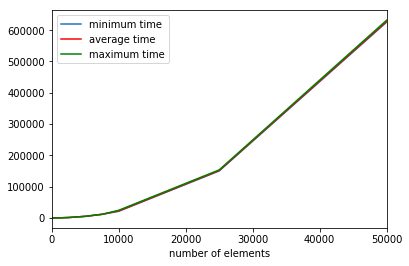
\includegraphics[scale=.75]{images/selectionsort.png}
\caption{Gráfico de desempenho do algoritmo Selection Sort}
\label{mapaSelection}
\end{figure}

\begin{figure}[H]
\centering
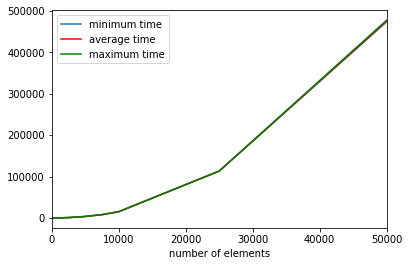
\includegraphics[scale=.75]{images/insertionsort.png}
\caption{Gráfico de desempenho do algoritmo Insertion Sort}
\label{mapaInsertion}
\end{figure}

\begin{figure}[H]
\centering
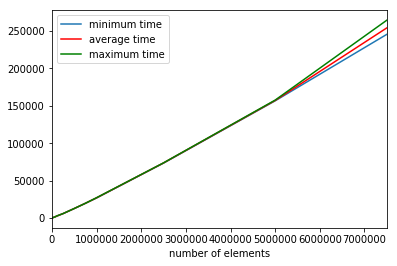
\includegraphics[scale=.75]{images/mergesort.png}
\caption{Gráfico de desempenho do algoritmo Merge Sort}
\label{mapaMerge}
\end{figure}

\begin{figure}[H]
\centering
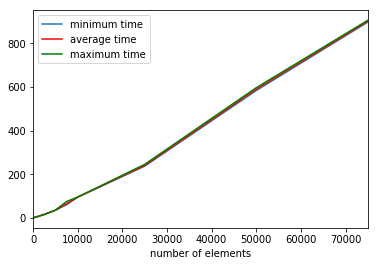
\includegraphics[scale=.75]{images/quicksort.png}
\caption{Gráfico de desempenho do algoritmo Quick Sort}
\label{mapaQuick}
\end{figure}

\begin{figure}[H]
\centering
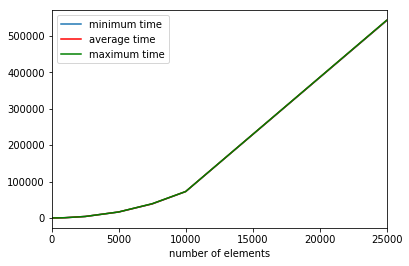
\includegraphics[scale=.75]{images/heapsort.png}
\caption{Gráfico de desempenho do algoritmo Heap Sort}
\label{mapaHeap}
\end{figure}

\begin{figure}[H]
\centering
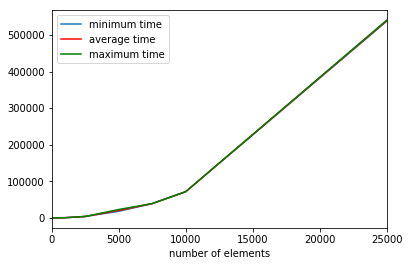
\includegraphics[scale=.75]{images/introsort.png}
\caption{Gráfico de desempenho do algoritmo Intro Sort}
\label{mapaIntro}
\end{figure}

\begin{figure}[H]
\centering
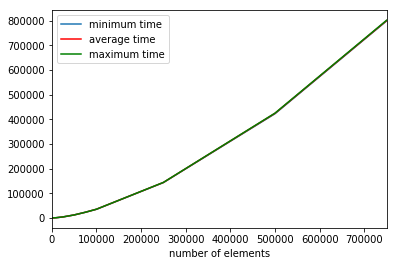
\includegraphics[scale=.75]{images/patiencesort.png}
\caption{Gráfico de desempenho do algoritmo Patience Sort}
\label{mapaPatience}
\end{figure}


\begin{figure}[H]
\centering
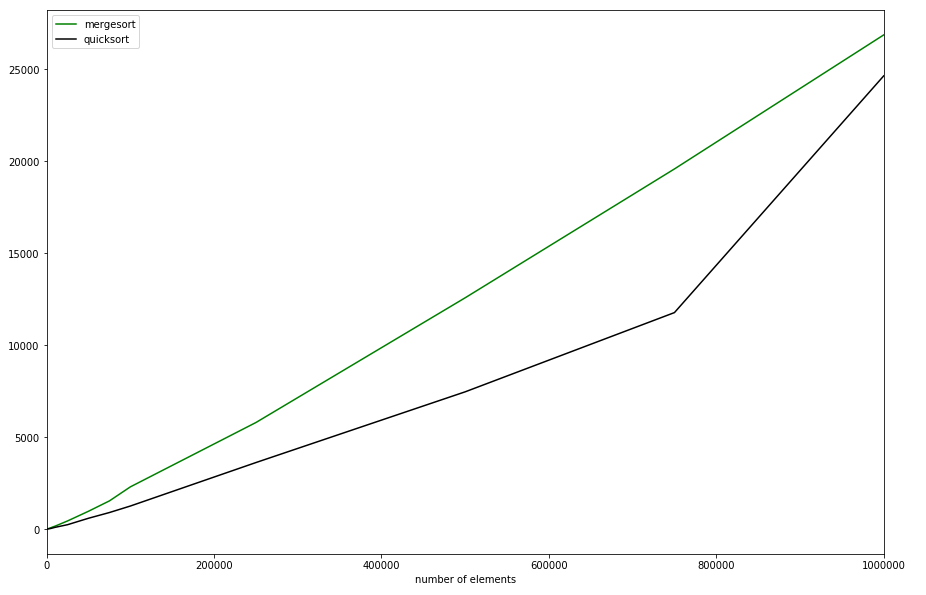
\includegraphics[scale=.70]{images/principais.png}
\caption{Gráfico de desempenho do merge e quick até 1.000.000 de entradas}
\label{mapaPrincipais}
\end{figure}

\begin{figure}[H]
\centering
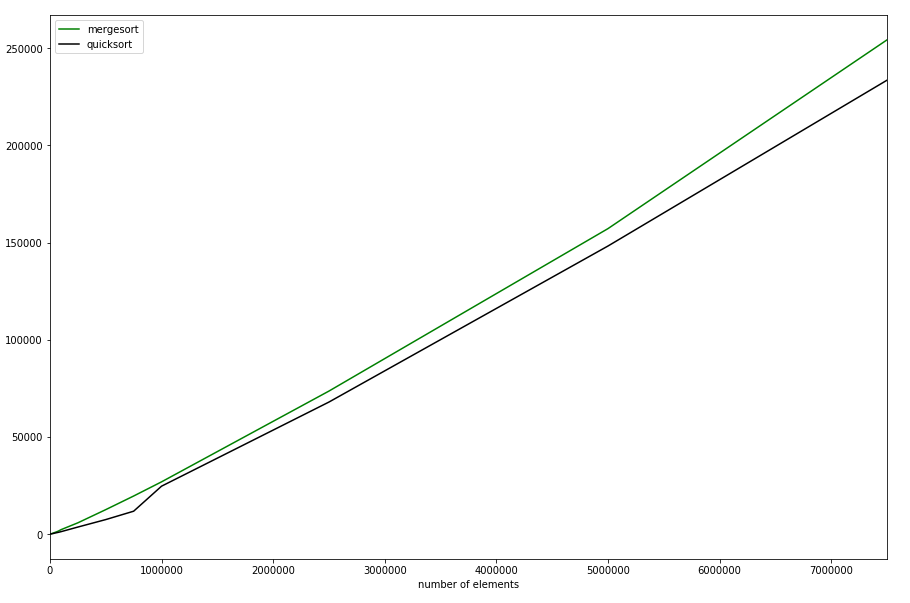
\includegraphics[scale=.70]{images/principais7M.PNG}
\caption{Gráfico de desempenho do merge e quick até 7.500.000 de entradas}
\label{mapaPrincipais}
\end{figure}

\begin{figure}[H]
\centering
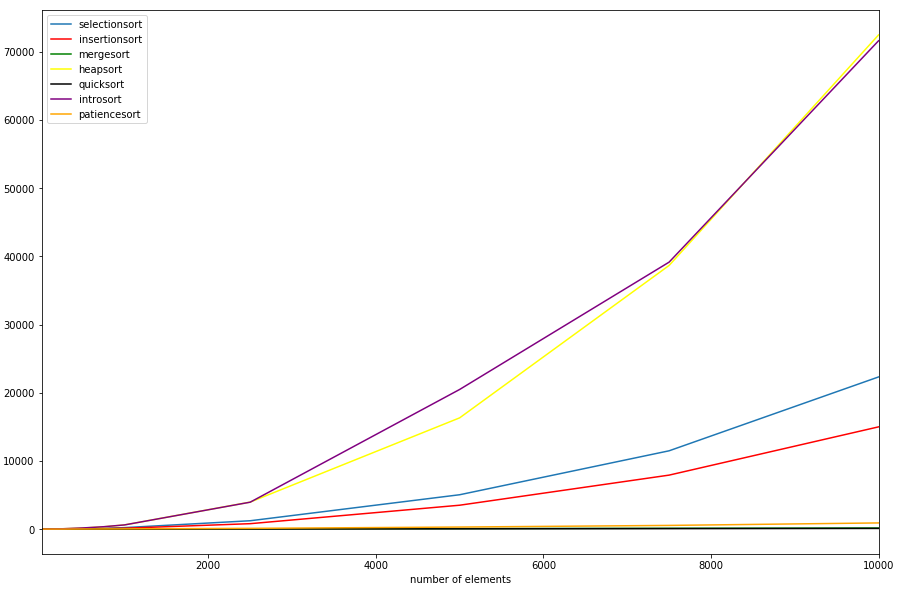
\includegraphics[scale=.70]{images/todos10.png}
\caption{Gráfico de todos algoritmos até 10.000 entradas}
\label{mapaPrincipais}
\end{figure}

\begin{figure}[H]
\centering
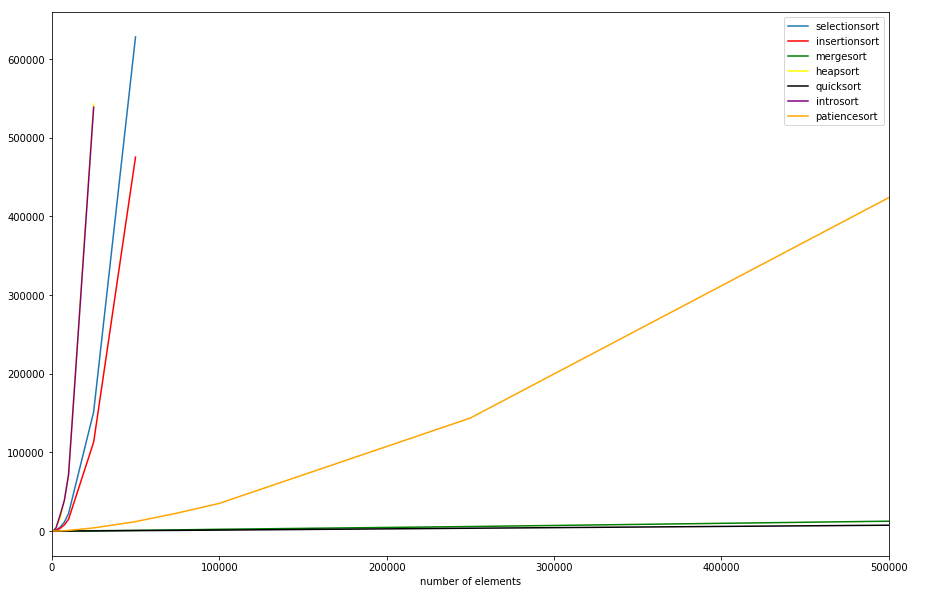
\includegraphics[scale=.70]{images/todos50.PNG}
\caption{Gráfico de todos algoritmos até 500.000 entradas}
\label{mapaPrincipais}
\end{figure}

\begin{figure}[H]
\centering
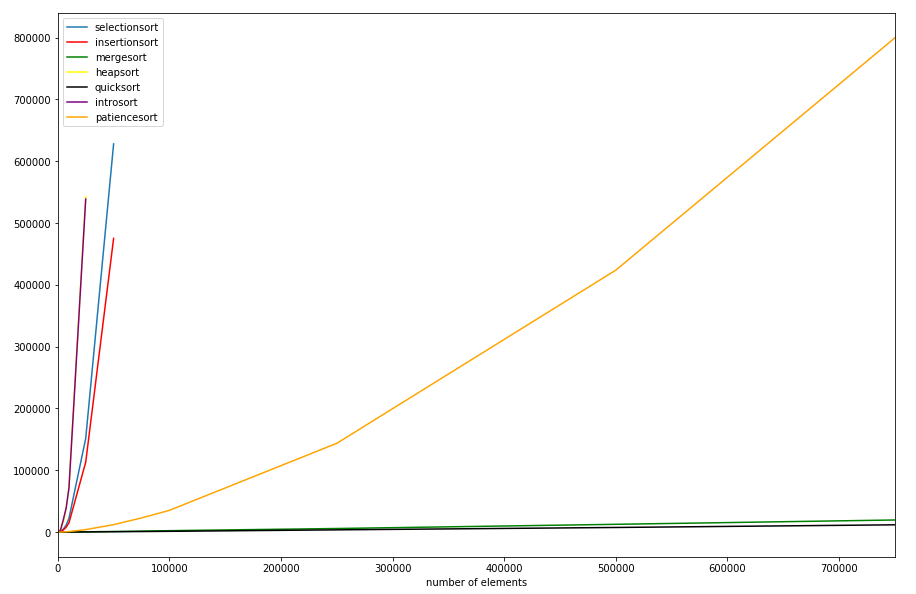
\includegraphics[scale=.70]{images/todos75.png}
\caption{Gráfico de todos algoritmos até 7.500.000 entradas}
\label{mapaPrincipais}
\end{figure}

\begin{table}[]
\begin{tabular}{|l|l|l|l|l|l|l|l|}
\hline
\textbf{Algoritmo} & selection & insertion & merge & quick & heap  & intro & patience  \\ \hline
10                 & 0.03          & 0.03          & 0.06      & 0.03      & 0.10      & 0.12      & 0.05      \\ \hline
25                 & 0.14          & 0.10          & 0.14      & 0.08      & 0.42      & 0.39      & 0.21      \\ \hline
50                 & 0.50          & 0.30          & 0.42      & 0.21      & 1.42      & 1.46      & 0.39      \\ \hline
75                 & 1.09          & 0.97          & 0.56      & 0.26      & 3.97      & 4.49      & 0.55      \\ \hline
100                & 1.89          & 1.95          & 0.78      & 0.34      & 7.19      & 8.18      & 0.96      \\ \hline
250                & 13.84         & 9.08          & 2.54      & 1.21      & 40.87     & 43.30     & 3.22      \\ \hline
500                & 57.20         & 36.51         & 5.65      & 3.16      & 151.30    & 166.80    & 12.18     \\ \hline
750                & 116.77        & 77.60         & 8.78      & 4.78      & 335.18    & 346.58    & 22.33     \\ \hline
1000               & 215.65        & 127.98        & 14.57     & 5.88      & 611.16    & 612.17    & 33.90     \\ \hline
2500               & 1223.70       & 793.61        & 34.78     & 15.80     & 3958.96   & 3946.46   & 107.81    \\ \hline
5000               & 5037.75       & 3502.10       & 73.49     & 35.36     & 16316.38  & 20479.75  & 299.94    \\ \hline
7500               & 11482.98      & 7916.35       & 121.21    & 65.26     & 38667.80  & 39154.64  & 539.47    \\ \hline
10000              & 22315.99      & 14993.89      & 159.51    & 95.37     & 72479.85  & 71622.42  & 903.81    \\ \hline
25000              & 151518.74     & 113106.48     & 445.03    & 240.27    & 542724.06 & 538826.69 & 4023.42   \\ \hline
50000              & 628121.48     & 475280.39     & 971.74    & 590.15    & -1        & -1        & 12044.46  \\ \hline
75000              & -1            & -1            & 1535.16   & 901.37    & -1        & -1        & 22918.33  \\ \hline
100000             & -1            & -1            & 2298.22   & 1255.20   & -1        & -1        & 35188.48  \\ \hline
250000             & -1            & -1            & 5797.74   & 3619.60   & -1        & -1        & 143673.68 \\ \hline
500000             & -1            & -1            & 12582.86  & 7467.44   & -1        & -1        & 423854.92 \\ \hline
750000             & -1            & -1            & 19591.12  & 11776.81  & -1        & -1        & 799607.33 \\ \hline
1000000            & -1            & -1            & 26881.54  & 24652.75  & -1        & -1        & -1        \\ \hline
2500000           & -1            & -1            & 73584.08  & 67939.91  & -1        & -1        & -1        \\ \hline
5000000           & -1            & -1            & 157162.86 & 148210.46 & -1        & -1        & -1        \\ \hline
7500000           & -1            & -1            & 254268.34 & 233521.91 & -1        & -1        & -1        \\ \hline
\end{tabular}
\caption{Tabela com os tempos correspondentes a cada arquivo em cada algoritmo. Para os valores iguais a -1, referem-se ao tempo superior a 15 minutos de execução}
\end{table}

\begin{table}[]
\begin{tabular}{|l|l|l|l|l|l|l|}
\hline
\textbf{} & 1º lugar & tempo     & 2º lugar & tempo     & 3º lugar & tempo     \\ \hline
10        & selection & 0.03      & insertion & 0.03      & quick     & 0.03      \\ \hline
25        & quick     & 0.08      & insertion & 0.10      & selection & 0.14      \\ \hline
50        & quick     & 0.21      & insertion & 0.3       & patience  & 0.39      \\ \hline
75        & quick     & 0.26      & patience  & 0.55      & merge     & 0.56      \\ \hline
100       & quick     & 0.34      & merge     & 0.78      & patience  & 0.96      \\ \hline
250       & quick     & 1.21      & merge     & 2.54      & patience  & 3.22      \\ \hline
500       & quick     & 3.16      & merge     & 5.65      & patience  & 12.18     \\ \hline
750       & quick     & 4.78      & merge     & 8.78      & patience  & 22.33     \\ \hline
1000      & quick     & 5.88      & merge     & 14.57     & patience  & 33.9      \\ \hline
2500      & quick     & 15.8      & merge     & 34.78     & patience  & 107.81    \\ \hline
5000      & quick     & 35.36     & merge     & 73.49     & patience  & 299.94    \\ \hline
7500      & quick     & 65.26     & merge     & 121.21    & patience  & 539.47    \\ \hline
10000     & quick     & 95.37     & merge     & 159.51    & patience  & 903.81    \\ \hline
25000     & quick     & 240.27    & merge     & 445.03    & patience  & 4023.42   \\ \hline
50000     & quick     & 590.15    & merge     & 971.74    & patience  & 12044.46  \\ \hline
75000     & quick     & 901.37    & merge     & 1535.16   & patience  & 22918.33  \\ \hline
100000    & quick     & 1255.2    & merge     & 2298.22   & patience  & 35188.48  \\ \hline
250000    & quick     & 3619.6    & merge     & 5797.74   & patience  & 143673.68 \\ \hline
500000    & quick     & 7467.44   & merge     & 12582.86  & patience  & 423854.92 \\ \hline
750000    & quick     & 11776.81  & merge     & 19591.12  & patience  & 799607.33 \\ \hline
1000000   & quick     & 24652.75  & merge     & 26881.54  &           &           \\ \hline
2500000  & quick     & 67939.91  & merge     & 73584.08  &           &           \\ \hline
5000000  & quick     & 148210.46 & merge     & 157162.86 &           &           \\ \hline
7500000  & quick     & 233521.91 & merge     & 254268.34 &           &           \\ \hline
\end{tabular}
\caption{Tabela com os 3 melhores algoritmos para cada tamanho de entrada}
\end{table}






\newpage
\section{Referências}

Cormen,T.C. et al. \textbf{Algoritimos: Teoria e prática}. 2º Edição Americana. \newline
\href{https://pt.wikipedia.org/wiki/Selection_sort}{Wikipedia - Selection Sort} \newline
\href{https://pt.wikipedia.org/wiki/Insertion_sort}{Wikipedia - Insertion Sort} \newline
\href{https://pt.wikipedia.org/wiki/Merge_sort}{Wikipedia - Merge Sort} \newline
\href{https://pt.wikipedia.org/wiki/Heapsort}{Wikipedia - Heap Sort} \newline
\href{https://en.wikipedia.org/wiki/Patience_sorting}{Wikipedia - Patience Sort} \newline
\href{https://pt.wikipedia.org/wiki/Intro_sort}{Wikipedia - Intro Sort} \newline
\href{http://queirozf.com/entries/pandas-dataframe-plot-examples-with-matplotlib-pyplot?fbclid=IwAR3wI3aBcqORDyV3vOBtEQ5Z9JP4-u7Q62iLRXbBLMW2LdGueavkDrCKsi0}{Pandas Dataframe: Plot Examples with Matplotlib and Pyplot} \newline
\href{https://tutorials.technology/tutorials/17-how-to-plot-with-python-pandas.html?fbclid=IwAR1AINNONWOc0w_Q4duRbv46GXBsSK2tFdcmXLWy2b-p641iU0YG2-DE1B4}{How To Plot With Python Pandas} \newline
\href{https://stackoverflow.com/questions/42372617/how-to-plot-csv-data-using-myplotlib-and-pandas-in-python?fbclid=IwAR1XKuZiii5LZpc1vocW91f-1WTsHfUdcaJrQznXvq74WE67e_RZcx3IqkM}{How To Plot CSV data using myplotlib and pandas in python} \newline
\href{https://medium.com/horadecodar/data-science-tips-02-como-usar-loc-e-iloc-no-pandas-fab58e214d87}{Pandas Dataframe: Como usar loc e iloc no pandas} \newline
\href{https://towardsdatascience.com/a-guide-to-pandas-and-matplotlib-for-data-exploration-56fad95f951c}{A guide to pandas and matplotlib for data exploration} \newline
\end{document}

% Local Variables:
% ispell-local-dictionary: "brasileiro"
% TeX-master: t
% TeX-command-extra-options: "-shell-escape"
% End: